\documentclass[tikz,border=10pt]{standalone}
\usepackage{tikz}
\usetikzlibrary{positioning, arrows.meta}




% Definición detallada de una llave
\tikzset{
  mykey/.pic={
    \fill[black] (0,0) circle (0.2);     
    \fill[white] (0,0) circle (0.05);
    \fill[black] (0.2,0) rectangle (0.75,0.08);
    \fill[black] (0.3,0) -- (0.35,-0.1) -- (0.4,0) -- cycle; 
    \fill[black] (0.45,0) -- (0.5,-0.1) -- (0.55,0) -- cycle; 
    \fill[black] (0.6,0) -- (0.65,-0.1) -- (0.7,0) -- cycle; 
  }
}

\begin{document}
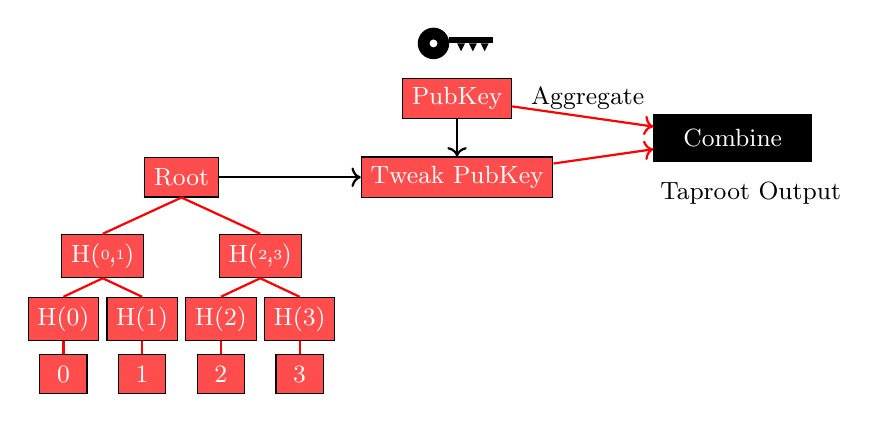
\begin{tikzpicture}[
    mast/.style={draw,fill=red!70,minimum width=0.6cm,minimum height=0.5cm,text=white},
    combined/.style={draw=black,fill=black,text=white,minimum width=2cm,minimum height=0.6cm},
    font=\small
  ]


  \foreach \i in {0,1,2,3} {
  \node[mast] (a\i) at (0+\i*1,0) {\i};
  \node[mast] (b\i) at (0+\i*1,0.7) {H(\i)};
  \draw[red, thick] (a\i.north) -- (b\i.south);
}

  \foreach \i in {0,1} {
  \node[mast] (c\i) at (0.5+\i*2,1.5) {H( , )};
}

  \node[anchor=west,font=\tiny,text=white] at (0.35,1.5) {0,1};  
  \node[anchor=west,font=\tiny,text=white] at (2.35,1.5) {2,3};
  \draw[red, thick] (c1.south) -- (b2.north);
  \draw[red, thick] (c1.south) -- (b3.north);
  \draw[red, thick] (c0.south) -- (b1.north);
  \draw[red, thick] (c0.south) -- (b0.north);
  \node[mast] (d) at (1.5,2.5) {Root};
  \draw[red, thick] (d.south) -- (c1.north);
  \draw[red, thick] (d.south) -- (c0.north);

  \node[mast] (tweak) at (5,2.5) {Tweak PubKey};
  \draw[->,black, thick] (d) -- (tweak);

   \node[mast] (pubkey) at (5,3.5) {PubKey};
   \draw[->,black, thick] (pubkey) -- (tweak);
   \pic at (4.7,4.2) {mykey};

    \node[combined] (combined) at (8.5,3) {Combine};
    \draw[->,red,thick] (pubkey) -- (combined);
    \draw[->,red,thick] (tweak) -- (combined);
    
    \node[anchor=east,font=\small] at (10,2.3) {Taproot Output};
    \node[anchor=east,font=\small] at (7.5,3.5) {Aggregate};

\end{tikzpicture}
\end{document}
